%==============================================================================
%    LATEX PREAMBLE  
%==============================================================================

\documentclass{article}
\usepackage[T1]{fontenc}
\usepackage{microtype}
\usepackage{graphicx}
\usepackage{subfigure}
\usepackage{booktabs} % for professional tables
\usepackage{hyperref, xcolor}
\usepackage{amsmath, amssymb, amsthm, hanging, graphicx, txfonts, ifthen}

\newcommand{\theHalgorithm}{\arabic{algorithm}}
\newtheorem{prop}{Proposition}

\usepackage{icml2019}
%\usepackage[accepted]{icml2019}

\usepackage{array}   % for \newcolumntype macro
\newcolumntype{L}{>{$}l<{$}}

\definecolor{moor}{rgb}{0.8,0.2,0.2}
\definecolor{moog}{rgb}{0.2,0.8,0.2}
\definecolor{moob}{rgb}{0.2,0.2,0.8}

\newcommand{\RR}{\mathbb{R}}
\newcommand{\expc}{\mathbb{E}}
\newcommand{\expct}[1]{\mathbb{E}\left[#1\right]}
\newcommand{\wrap}[1]{\left( #1 \right)}
\newcommand{\wang}[1]{\left\langle #1 \right\rangle}
\newcommand{\wive}[1]{\left\llbracket #1 \right\rrbracket}
\newcommand{\worm}[1]{\left\| #1 \right\|}

\newcommand{\dia}[1] {\begin{gathered}\includegraphics[scale=0.2 ]{../diagrams/#1.png}\end{gathered}}
\newcommand{\mdia}[1]{\begin{gathered}\includegraphics[scale=0.16]{../diagrams/#1.png}\end{gathered}}
\newcommand{\sdia}[1]{\begin{gathered}\includegraphics[scale=0.12]{../diagrams/#1.png}\end{gathered}}

    

\newcommand{\half}{\frac{1}{2}}
\newcommand{\sixth}{\frac{1}{6}}

\newcommand{\ofsix}[1]{
    {\tiny $\substack{
        \ifthenelse{\equal{#1}{0}}{\blacksquare}{\square}
        \ifthenelse{\equal{#1}{1}}{\blacksquare}{\square}
        \ifthenelse{\equal{#1}{2}}{\blacksquare}{\square}\\
        \ifthenelse{\equal{#1}{3}}{\blacksquare}{\square}
        \ifthenelse{\equal{#1}{4}}{\blacksquare}{\square}
        \ifthenelse{\equal{#1}{5}}{\blacksquare}{\square}
    }$}
}


\newcommand{\lorem}[1]{
    Lorem ipsum dolor sit amet, consectetur adipiscing elit...\\
    \nopagebreak\vspace{#1cm} \ \\
    ...sunt in culpa qui officia deserunt mollit anim id est laborum.
}


\begin{document}

%==============================================================================
%    TITLE AND AUTHOR
%==============================================================================

\icmltitlerunning{Descent as Scattering}

\twocolumn[
    \icmltitle{A Space-Time Approach to Analyzing Stochastic Gradient Descent}
    
    \begin{icmlauthorlist}
        \icmlauthor{Samuel C.~Tenka}{mit}
    \end{icmlauthorlist}
    \icmlaffiliation{mit}{
        Computer Science and Artificial Intelligence Lab,
        Massachusetts Institute of Technology,
        Cambridge, Massachusetts, USA
    }
    \icmlcorrespondingauthor{Samuel C.~Tenka}{coli@mit.edu}
    
    \icmlkeywords{Machine Learning, SGD, ICML}
    
    \vskip 0.3in
]
\printAffiliationsAndNotice{}

%==============================================================================
%    ABSTRACT        
%==============================================================================

\begin{abstract}
    We present a diagrammatic calculus for reasoning about the behavior, at
    small learning rates, of SGD and its variants.  We interpret the diagrams
    as histories of scattering events, thus offering a new physical analogy for
    descent.  Illustrating this technique, we construct a regularizing term
    that causes large-batch GD to emulate small-batch SGD, present a
    model-selection heuristic that depends only on statistics measured before
    optimization, and exhibit a counter-intuitive loss landscape wherein SGD
    eternally cycles counterclockwise around a circle of minima. 
\end{abstract}

%==============================================================================
%    INTRODUCTION    
%==============================================================================
\section{Introduction}
    Stochastic gradient descent (SGD) decreases an unknown objective $l$ by
    performing discrete-time steepest descent on noisy estimates of $l$.  A key
    question is how the noise affects the final objective value.  We connect
    SGD dynamics to physical scattering theory, thus providing a quantitative
    and qualitative toolkit for answering this question.

    Specifically, we derive a diagram-based formalism for reasoning about SGD
    via a path integral over possible interactions between weights and data.
    The formalism permits perturbative analysis, leading to predictions of
    learning curves for small $\eta$.  Unlike the continuous-time limits of
    previous work, this framework models discrete time, and with it, the
    potential {\bf non-Gaussianity} of noise.  We thus obtain new results
    quantifying the {\bf effect of epoch number, batch size, and momentum} on
    SGD test loss.  We also contrast SGD against popular continuous-time
    approximations such as ordinary or stochastic differential equations (ODE,
    SDE).
    
    Path integrals offer not only quantitative predictions but also an exciting
    new viewpoint --- that of iterative optimization as a {\bf scattering
    process}.  Much as individual Feynman diagrams (see \citet{dy49a}) depict
    how local particle interactions compose into global outcomes, our diagrams
    depict how individual SGD updates influence each other before affecting a
    final test loss.  In fact, we import from physics tools such as {\bf
    crossing symmetries} (see \citet{dy49b}) and {\bf re-normalization} (see
    \citet{ge54}) to simplify our calculations and refine our estimates.
    The diagrams' combinatorial properties immediately yield several precise
    qualitative conclusions as well, for instance that to order $\eta^2$, {\bf
    inter-epoch} shuffling does not affect expected test loss.

%==============================================================================
%    BACKGROUND AND NOTATION
%==============================================================================

\section{Background and Notation}

\subsection*{Gradient-Based Optimization and Generalization}
    We adopt the standard summation notation for Greek but not Roman indices,
    suppressing indices when convenient and clear.  To expedite dimensional
    analysis, we follow \cite{bo13} in considering the learning rate as an
    inverse metric $\eta^{\mu\nu}$ that converts a gradient (row vector) into a
    displacement (column vector).

    Then SGD with learning rate $\eta^{\mu\nu}$ decreases an objective $l$ by
    updating on a sequence of smooth, unbiased i.i.d.  estimates $(l_n: 0\leq
    n<N)$ of $l$:
    \begin{equation}\label{eq:sgdstep} \theta_{t+1} \coloneqq \theta_t -
        \eta^{\mu\nu} \nabla_\mu l_t(\theta_t)~~~~~~~~~~~~~(0\leq t<T=N)
    \end{equation}

    \lorem{5}

\subsection*{Motivating Example}
    Gradient descent makes a first order approximation
    {\color{red} FILL IN}

    Intuitively, each descent step displaces $\theta$ by $-\eta \nabla l$ and
    hence decreases the loss $l(\theta)$ by $\eta (\nabla l)^2$; thus, we
    expect after $T$ steps a net decrease of $T \eta (\nabla l)^2$:
    \begin{equation} \label{eq:motone}
        l(\theta_T) \approx l(\theta_0) - T \cdot \eta \cdot (\nabla l(\theta_0))^2
    \end{equation}
    This intuition fails to capture two crucial facts: {\bf curvature} --- that
    as $\theta$ changes during training, so may $\nabla l(\theta)$ --- and {\bf
    noise} --- that $l_n$ and $l$ may differ.
    %
    We may account for curvature, i.e. $\nabla \theta$'s evolution, in analogy
    with (\ref{eq:motone})'s estimate of $l(\theta)$'s evolution: each step
    displaces $\theta$ by $-\eta(\nabla l)$ and hence changes $\nabla
    l(\theta)$ by $-\eta (\nabla^2 l) (\nabla l)$; thus, we expect that $\nabla
    l(\theta_t)$ differs from $l(\theta_0)$ by $-t \eta (\nabla^2 l) (\nabla
    l)$.  Recalling that $\sum_{0\leq t<T} t = {T \choose 2}$, we estimate the
    net displacement of $\theta$ as $\Delta \theta = -T \eta \nabla l + {T
    \choose 2} \eta^2 (\nabla^2 l) (\nabla l)$.  We thus refine
    (\ref{eq:motone}) by substituting $\Delta \theta$ into a Taylor expansion
    of $l$ at $\theta_0$ ($l, \cdots$ unadorned are evaluated at $\theta_0$):
    \begin{align} \label{eq:mottwo}
        l(\theta_T)
        \approx l +& \wrap{-T \eta \nabla l + {T \choose 2} \eta^2 (\nabla^2 l) (\nabla l)} \nabla l \\
                  +& \frac{1}{2} \wrap{-T \eta \nabla l + {T \choose 2} \eta^2 (\nabla^2 l) (\nabla l)}^2 \nabla l^2 \\
        \approx l -& T \cdot \eta \cdot \wrap{\nabla l}^2 \\
                  +& T \wrap{T-\frac{1}{2}} \cdot \eta^2 \cdot \nabla^2 l (\nabla l)^2
    \end{align}
    So far, we have essentially recovered Theorem 2.1.14 of \citet{ne04}.
    
    After establishing some general-purpose results, we will be able to
    {\color{red} FILL IN}. 
    
    The more complicated the direct computation, the greater the savings of
    using diagrams.
        
\subsection*{Physical Dictionary}

%==============================================================================
%    DIAGRAM CALCULUS FOR SGD
%==============================================================================

\section{Diagram Calculus for SGD}
\subsection*{Role of Diagrams}
    Suppose $s$ is smooth on weight space; for example, $s$ may be a test or
    train loss.  We may track $s(\theta)$ as $\theta$ is updated by SGD as
    follows:
    \begin{prop}
        The formal Maclaurin series of $s(\theta_T)$ with respect to $\eta$ is:
        \begin{equation*}\label{eq:dyson}
            \sum_{0\leq d < \infty} (-\eta)^d \sum_{\substack{(d_t: 0\leq t<T) \\ \sum_t d_t = d}}
            \left(
                \prod_{0 \leq t < T}
                    \left.  \frac{(g \nabla)^{d_t}}{d_t!} \right|_{g=\nabla l_t(\theta)}
            \right)
            s (\theta_0)
        \end{equation*}
    \end{prop}
    In averaging over training sets (and hence over the sequence $(l_t: 0\leq
    t<T)$ considered as a random variable), we may factor the expectation of
    the above product according to independence relations between the $l_t$.
    We view various training procedures (e.g. GD, SGD with(out) inter-epoch
    shuffling) as {\bf prescribing different independence relations} that lead
    to different factorizations and hence to potentially different
    generalization behavior at each order of $\eta$.

    An instance of the above product (for $s=l_a$ drawn from a test set and
    $0\leq c\leq b<T$) is \begin{align*}
        \eta^3 (\nabla l_c \nabla)^2 (\nabla l_b \nabla) l_a
        = & & (\nabla^\lambda l_c) (\nabla^\mu l_c) (\nabla_\lambda \nabla_\mu \nabla^\nu l_b) (\nabla_\nu l_a) \\
          &+& (\nabla^\lambda l_c) (\nabla^\mu l_c) (\nabla_\lambda \nabla^\nu l_b) (\nabla_\mu \nabla_\nu l_a) \\
          &+& (\nabla^\lambda l_c) (\nabla^\mu l_c) (\nabla_\mu \nabla^\nu l_b) (\nabla_\lambda \nabla_\nu l_a) \\
          &+& (\nabla^\lambda l_c) (\nabla^\mu l_c) (\nabla^\nu l_b) (\nabla_\lambda \nabla_\mu \nabla_\nu l_a)
    \end{align*}
    where we use $\eta$ to raise indices.  To reduce clutter, we adapt the
    string notation of \citet{pe71}.  Then, in expectation over $(l_c, l_b,
    l_a)$ drawn i.i.d.:
    \begin{align*}
        \cdots
        &= 
             \sdia{(01-2-3)(02-12-23)}
            +\sdia{(01-2-3)(02-13-23)}
            +\sdia{(01-2-3)(03-12-23)}
            +\sdia{(01-2-3)(03-13-23)} \\
        &=
            \underbrace{2\sdia{(01-2-3)(02-12-23)}}_{
                2~\expct{{\color{moor}(\nabla l)(\nabla l)}}~\expct{{\color{moog}\nabla\nabla\nabla l}}~\expct{{\color{moob} \nabla l}}
            }
            +
            \underbrace{2\sdia{(01-2-3)(02-13-23)}}_{
                2~\expct{{\color{moor}(\nabla l)(\nabla l)}}~\expct{{\color{moog}\nabla \nabla l}}~\expct{{\color{moob}\nabla \nabla l}}
            }
    \end{align*}
    Above, each node corresponds to a loss function (here, red for $l_c$, green
    for $l_b$, blue for $l_a$), differentiated $d$ times for a degree-$d$ node
    (for instance, $l_b$ is differentiated thrice in the first diagram and
    twice in the second).  {\bf Thin ``edges''} mark contractions by $\eta$.
    {\bf Fuzzy ``ties''} denote independence relationships by connecting
    identical loss functions (here, $l_c$ with $l_c$): nodes not connected by a
    path of fuzzy ties are independent.  The colors are redundant with the
    fuzzy ties and used only so that we may concisely refer to a specific node
    in prose.  Crucially, for a fixed, i.i.d. distribution over $(l_c, l_b,
    l_a)$, {\bf the topology of a diagram determines its expected value}.  For
    instance, $\expc \sdia{(01-2-3)(02-12-23)} = \expc
    \sdia{(01-2-3)(03-13-23)}$ because both are trees with two leaves tied.
    Thus follows the simplification on the second line above.  As shown with
    braces, we may convert back to explicit tensor expressions, invoking
    independence between untied nodes to factor the expression.  However, as we
    will see, the diagrammatic form of a tensor expression offers us physical
    intuition and guides us toward constructing unbiased estimators of the
    statistics they represent.  
    
    The recipes for writing down test (or train) losses of SGD (or GD and other
    variants) are straight-forward in the diagram notation because they reduce
    the problem of evaluating the previous dynamical expressions to the problem
    of counting isomorphic graphs.  An appendix provides details and proofs for
    a variety of instances.  For now, we illustrate how to compute the test
    loss of vanilla SGD.

\subsection*{Recipe for the Test Loss of Vanilla SGD}
    The diagrams relevant to order $(-\eta)^d$ of this Taylor expansion are
    trees with $d$ thin edges, none of which connect fuzzily-tied nodes, and
    such that the rightmost node is not fuzzily tied.  We regard a diagram as a
    partial order (by reading the thin edges as Hasse diagram) equipped with a
    partition of nodes (induced by the fuzzy ties).  If a diagram's nodes
    partition into $P$ sets of size $(d_p: 0\leq p < P)$, then the Taylor
    coefficient on that diagram's isomorphism class is
    $$
        \frac{(-\eta)^d}{d!} {T \choose P} {d \choose d_0, \cdots, d_{P-1}}
        \cdot 
        K_{D \to [d+1]}
        \in
        \Theta\left((\eta T)^d T^{P-d-1}\right)
    $$
    where $K_{D \to [d+1]}$ counts the total orders that extend the partial
    order of $D$ and in which each of the $P$ parts appears as a contiguous
    segment.  For example, at order $(-\eta)^3 {T \choose 3}$ there are two
    isomorphism classes respectively with $4$ and $2$ total orderings,
    respectively; at order $(-\eta)^3 {T \choose 2}$ there are three classes
    respectively with $2$, $2$, and $3$ orderings; at order $(-\eta)^3 {T
    \choose 1}$ there is only one class and it has $1$ ordering (see Table
    \ref{tab:scatthree}).
    \begin{table}[h!]
        \centering 
        \resizebox{\columnwidth}{!}{%
        \begin{tabular}{c|c|c}
            %$\frac{(-\eta)^3}{3!} {T \choose 3} {3 \choose 1, 1, 1} $ &
            %$\frac{(-\eta)^3}{3!} {T \choose 2} {3 \choose 1, 2}    $ &
            %$\frac{(-\eta)^3}{3!}{T \choose 1} {3 \choose 3}        $ \\ & & \\
            $\Theta\left((\eta T)^3 T^{-0}\right)$ &
            $\Theta\left((\eta T)^3 T^{-1}\right)$ &
            $\Theta\left((\eta T)^3 T^{-2}\right)$ \\ \hline
            \begin{tabular}{c}
                \begin{tabular}{LL}
                    \dia{(0-1-2-3)(01-12-23)} & \dia{(0-1-2-3)(01-13-23)}
                \end{tabular} \\
                \begin{tabular}{LL}
                    \dia{(0-1-2-3)(02-13-23)} & \dia{(0-1-2-3)(03-12-23)}
                \end{tabular} \\ \hline
                \begin{tabular}{LL}
                    \dia{(0-1-2-3)(03-13-23)} & \dia{(0-1-2-3)(02-12-23)}
                \end{tabular}
            \end{tabular}
            &
            \begin{tabular}{c}
                \begin{tabular}{LL}
                    \dia{(01-2-3)(02-13-23)} & \dia{(01-2-3)(03-12-23)}
                \end{tabular} \\ \hline
                \begin{tabular}{LL}
                    \dia{(0-12-3)(01-13-23)} & \dia{(0-12-3)(02-13-23)}
                \end{tabular} \\ \hline
                \begin{tabular}{LLL}
                    \dia{(01-2-3)(03-13-23)} & \dia{(0-12-3)(03-13-23)} & \dia{(01-2-3)(02-12-23)} 
                \end{tabular}
            \end{tabular}
            &
            \begin{tabular}{c}
                \begin{tabular}{L}
                    \dia{(012-3)(03-13-23)}
                \end{tabular}
            \end{tabular}
        \end{tabular}
        }
        \caption{
            Degree-$3$ scattering diagrams for test loss of vanilla SGD.
            {\bf Left:} $(d, P) = (3, 3)$.  Diagrams for ODE behavior.
            {\bf Center:} $(d, P) = (3, 2)$.  $1$st order deviation of SGD away from ODE.
            {\bf Right:} $(d, P) = (3, 1)$.  $2$nd order deviation of SGD from ODE with appearance of
            non-Gaussian statistics.
        }
        \label{tab:scatthree}
    \end{table}
    Intuitively, we regard $\eta T$ as measuring the total {\bf physical time} of the optimization process, and
    $1/T$ as measuring the {\bf coarseness} of time discretization.  More precisely, we have a double-series in
    $(\eta T)^d T^{P-d-1}$, where $d$ counts thin edges and $d+1-P$ counts fuzzy ties; the $P=d+1$ terms give us an ODE (hence noiseless) approximation
    to SGD, while $P\leq d$ terms give us the effect of time-discretization and hence noise on SGD test loss.
    For Gaussian gradients,
    $\sdia{(012-3)(03-13-23)} = 3 \sdia{(01-2-3)(03-13-23)} - 2 \sdia{(0-1-2-3)(03-13-23)}$
    in expectation, but above, we make no such assumption.

\subsection*{Crossing Symmetries and Renormalization}
    \lorem{5}
    \lorem{5}

\subsection*{Descent as Scattering: Experimental}
    \lorem{5}
    \lorem{5}

%==============================================================================
%    PREDICTIONS AND APPLICATIONS
%==============================================================================

\section{Predictions and Applications}

    For single-epoch SGD with singleton batches, we sum all relevant diagrams through order $3$; the 
    coefficients $4, 2; 2, 2, 3; 1$ come from counting the elements of Table \ref{tab:scatthree}, and 
    the other coefficients come from analogous tables.  This yields:
    \begin{align*}
            &\mathcal{L}^{\text{SGD}}_\text{test}(T, \eta) \in                   
        \\ 
               \sdia{(0)()}
            &- \frac{\eta}{1!}   {T \choose 1} \wrap{\sdia{(0-1)(01)}}
        \\
            &+ \frac{\eta^2}{1!1!} {T \choose 2} \wrap{2 \sdia{(0-1-2)(01-12)}} 
             + \frac{\eta^2}{2!} {T \choose 1} \wrap{\sdia{(01-2)(02-12)}}
        \\
            &- \frac{\eta^3}{1!1!1!} {T \choose 3} \wrap{
                       4 \sdia{(0-1-2-3)(01-12-23)}+
                       2 \sdia{(0-1-2-3)(03-13-23)}
                   }
        \\
            &- \frac{\eta^3}{2!1!} {T \choose 2} \wrap{
                       2         \sdia{(01-2-3)(03-12-23)}+
                       2    \sdia{(0-12-3)(02-13-23)}+
                       3     \sdia{(01-2-3)(02-12-23)}
                   }
        \\
            &- \frac{\eta^3}{3!} {T \choose 1} \wrap{\sdia{(012-3)(03-13-23)}}
            + o(\eta^3)\footnotemark
    \end{align*}
    \footnotetext{
        We use little-$o(\eta^d)$ instead of big-$O(\eta^{d+1})$ to avoid specializing to analytic functions.
        Error terms depend on the loss landscape and on $T$.  When gradients are uniformly bounded,
        the $T$ dependence is at most linear.
    }
    By contrast, the generalization gap $\mathcal{L}^{\text{SGD}}_\text{gen} =
    \mathcal{L}^{\text{SGD}}_\text{test} -
    \mathcal{L}^{\text{SGD}}_\text{train}$ is suppressed by a factor $1/N$ ($N
    \leq T$):
    \begin{align*}
        &N \cdot \mathcal{L}^{\text{SGD}}_\text{gen}(T, \eta) \in
        \\
        &+ \eta   {T \choose 1} \wrap{\sdia{(01)(01)} - \sdia{(0-1)(01)}} 
        - \eta^2 {T \choose 2} \wrap{\sdia{(01-2)(01-12)} + \sdia{(02-1)(01-12)}- 2\sdia{(0-1-2)(01-12)}} \\
        &- \frac{\eta^2}{2!} {T \choose 1} \wrap{\sdia{(012)(02-12)} - \sdia{(01-2)(02-12)}} 
         + o(\eta^2) 
        %\\
        %=&+ \eta^{\lambda \mu} {T \choose 1} C_{\lambda \mu} 
        %- \eta^{\lambda \mu} \eta^{\nu \xi} {T \choose 2} \wrap{ \frac{1}{2} G_\lambda \nabla_\mu C_{\nu \xi} + C_{\mu \nu} H_{\xi \lambda} }
        %\\
        %&- \frac{\eta^{\lambda \mu} \eta^{\nu \xi}}{2!} {T \choose 1} \wrap{ \wang{l_\lambda l_\nu l_{\mu \xi}} - (G_{\mu}G_{\nu} + C_{\mu\nu})H_{\xi \lambda} }
        % + o(\eta^2) \\
    \end{align*}
    The leading order term is $N \cdot \mathcal{L}^{\text{SGD}}_\text{gen}(T, \eta) \approx \eta T \wrap{\sdia{(01)(01)} - \sdia{(0-1)(01)}} = T \cdot \eta^{\lambda\mu} C_{\lambda\mu}$,
    where $C$ is the covariance of gradients.  We thus recover a main result of \citet{ro18}.
    \begin{figure}[h!]
        \centering
        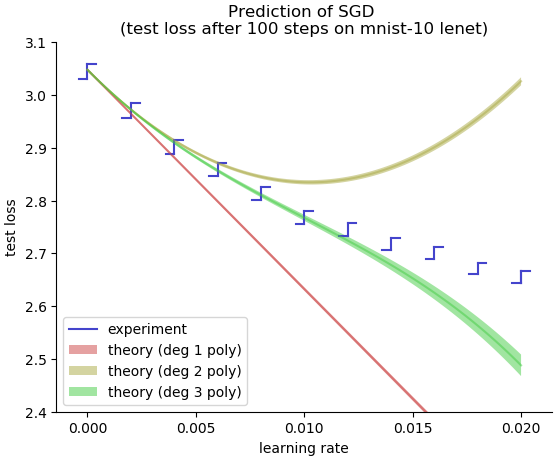
\includegraphics[width=4.0cm, trim={0 0 0 1.0cm}, clip]{test-lenet-07-poly}
        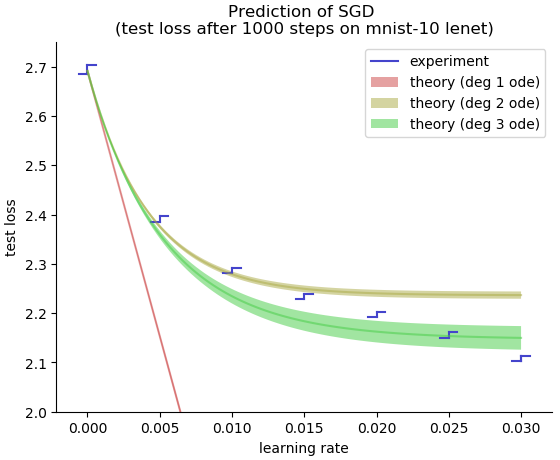
\includegraphics[width=4.0cm, trim={0 0 0 1.0cm}, clip]{test-lenet-long-06-ode} \\
        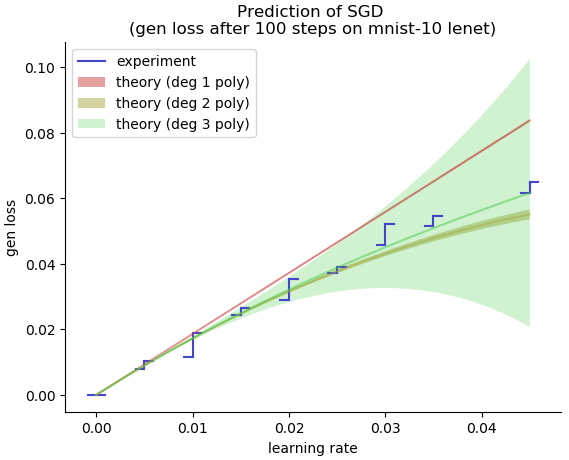
\includegraphics[width=4.0cm, trim={0 0 0 1.0cm}, clip]{gene-lenet-02-poly} 
        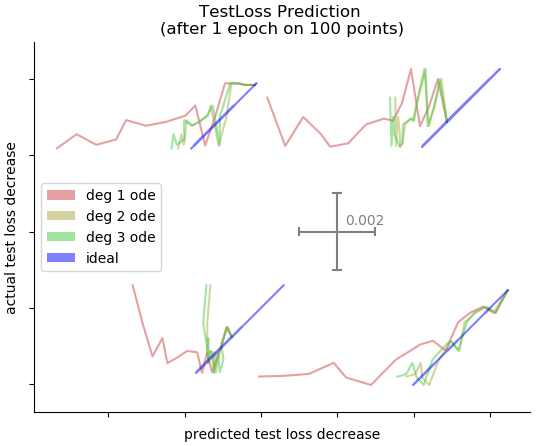
\includegraphics[width=4.0cm, trim={0 0 0 1.0cm}, clip]{test-loss-converged} \\
        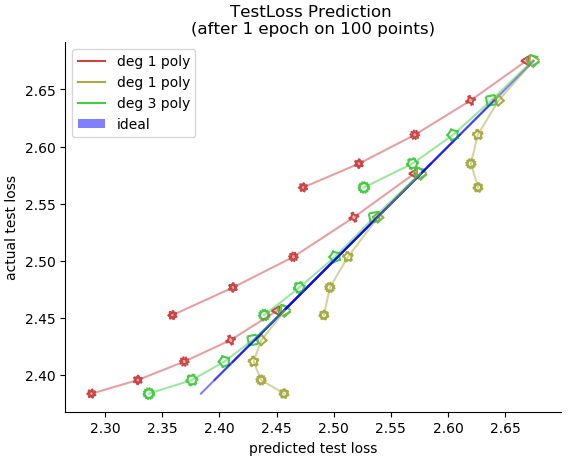
\includegraphics[width=4.0cm, trim={0 0 0 1.0cm}, clip]{test-loss}
        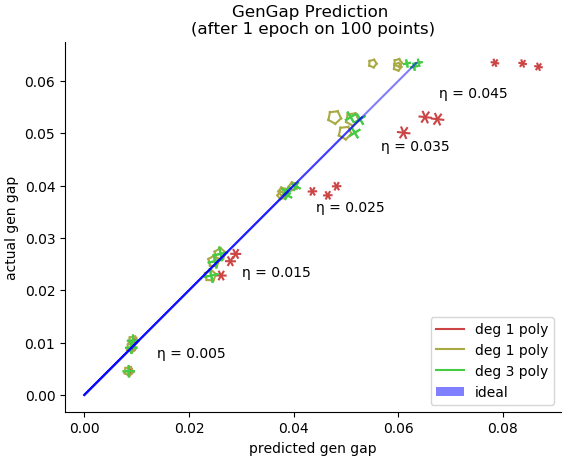
\includegraphics[width=4.0cm, trim={0 0 0 1.0cm}, clip]{gen-gap}
        \caption{
            MNIST-10 LeNet mean losses vs $\eta$ for $T=100$.   Top row's vertical spreads denote $95\%$
            confidence intervals.
            {\bf \ofsix{0}:} Test loss, polynomial fit.
            {\bf \ofsix{1}:} Test loss for larger $T=1000$, autonomous-ODE fit.
            {\bf \ofsix{2}:} Gen gap for a Xavier init.
            {\bf \ofsix{3}:} Test loss decrease for multiple inits near minima: actual vs predicted. 
            {\bf \ofsix{4}:} Test loss for multiple Xavier inits: actual vs predicted.
            {\bf \ofsix{5}:} Gen gap for multiple Xavier inits: actual vs predicted. {\color{red} axes transposed?!}
        }
        \label{fig:basic}
    \end{figure}
    \lorem{5}
       

\subsection*{Emulating Small Batches with Large Ones}
    \lorem{5}
    \lorem{5}

\subsection*{Analyzing Second Order Methods}
    \lorem{5}
    \lorem{5}

\subsection*{Epochs and Overfitting}
    \lorem{5}
    \lorem{5}

\subsection*{Myopic Model Selection}
    \lorem{3}
    \begin{figure}[h!]
        \centering
        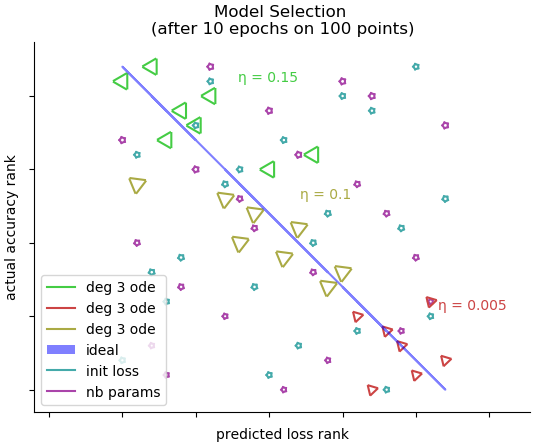
\includegraphics[width=4.0cm, trim={0 0 0 1.0cm}, clip]{model-selection-acc}
        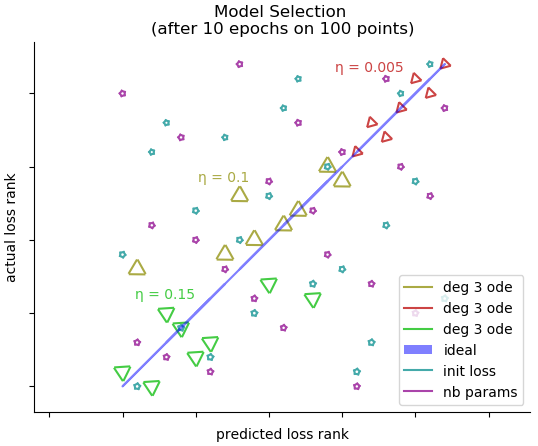
\includegraphics[width=4.0cm, trim={0 0 0 1.0cm}, clip]{model-selection-loss} \\
        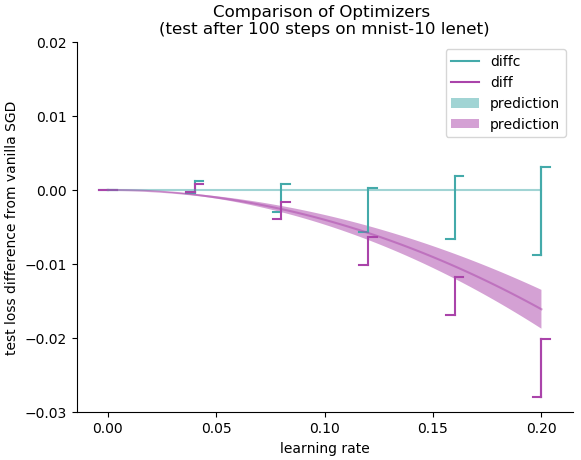
\includegraphics[width=4.0cm, trim={0 0 0 1.0cm}, clip]{batchmatch-06} 
        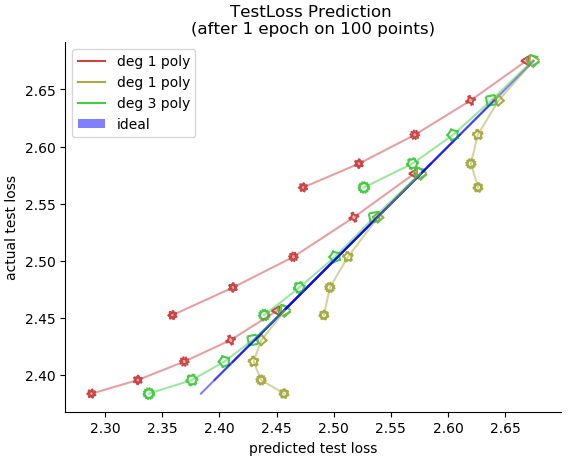
\includegraphics[width=4.0cm, trim={0 0 0 1.0cm}, clip]{test-loss} \\
        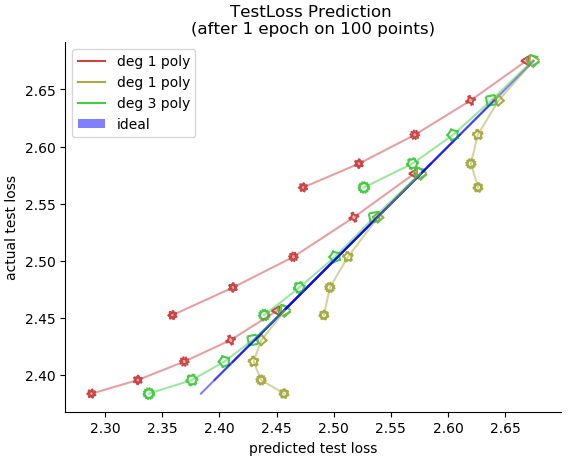
\includegraphics[width=4.0cm, trim={0 0 0 1.0cm}, clip]{test-loss} 
        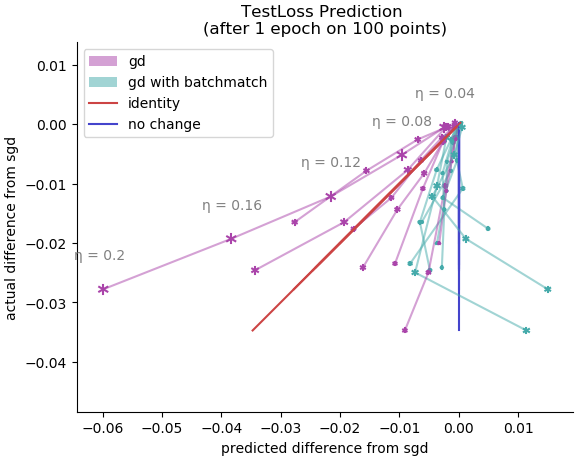
\includegraphics[width=4.0cm, trim={0 0 0 1.0cm}, clip]{test-loss-bm}
        \caption{
            Applications illustrated on MNIST LeNet.  Top row's vertical spreads denote $95\%$
            confidence intervals.
            {\bf \ofsix{0}:} Ranking architectures for high {\bf accuracy} by predicting optimized loss from init statistics.
            {\bf \ofsix{1}:} Ranking architectures for low {\bf loss} by predicting optimized loss from init statistics.
            {\bf \ofsix{2}:} Batch matching for a Xavier init.
            {\bf \ofsix{3}:} {\color{red} FILL IN!}
            {\bf \ofsix{4}:} {\color{red} FILL IN!}
            {\bf \ofsix{5}:} Batch matching for multiple Xavier inits: actual vs predicted.
        }
        \label{fig:basic}
    \end{figure}
    \lorem{5}
    \lorem{5}

\subsection*{Comparison to Continuous Time}
    \lorem{5}
    \lorem{5}

\subsection*{Thermodynamic Engine}
    We clarify  
    \lorem{5}
    \lorem{5}

%==============================================================================
%    RELATED WORK    
%==============================================================================

\section{Related Work}
    It was \citet{ki52} who, in uniting gradient descent \citep{ca47} with
    stochastic approximation \citep{ro51}, invented SGD.  Since the development
    of back-propagation for efficient differentiation \citep{we74}, SGD and its
    variants have been used to train connectionist models including neural
    networks \citep{bo91}, in recent years to remarkable success \citep{le15}.

    Several lines of work predict the overfitting of SGD-trained networks
    \citep{ne17a}.  For instance, \citet{ba17} controls the Rademacher
    complexity of deep hypothesis classes, leading to generalization bounds
    that are post hoc or optimizer-agnostic.  However, since deep networks
    trained via SGD generalize despite their seeming ability to shatter large
    sets \citep{zh17}, one infers that generalization arises from the aptness
    to data of not only architecture but also optimization \citep{ne17b}.
    Others have focused on the implicit regularization of SGD itself, for
    instance by modeling descent via stochastic differential equations (e.g.
    \citet{ch18}).  However, as explained by \citet{ya19}, such continuous-time
    analyses cannot treat covariance correctly, and so they err when
    interpreting results about SDEs as results about SGD.

    Following \citet{ro18}, we avoid making a continuous-time approximation by
    instead Taylor-expanding around the learning rate $\eta=0$.  In fact, we
    develop a diagrammatic language for evaluating each Taylor term that is
    similar to and inspired by the field theory methods popularized by
    \citet{dy49a}.  Using this technique, we quantify the overfitting effects
    of batch size and epoch number, and based on this analysis, propose a
    regularizing term that causes large-batch GD to emulate small-batch SGD,
    thus establishing a precise version of the
    Covariance-BatchSize-Generalization relationship conjectured in
    \citet{ja18}.  
    
    While we make rigorous, architecture-agnostic predictions of learning
    curves, these predictions become vacuous for large $\eta$.  Other
    discrete-time dynamical analyses allow large $\eta$ by treating neural
    generalization phenomenologically, whether by fitting to an
    empirically-determined correlate of Rademacher bounds \citep{li18}, by
    exhibiting generalization of local minima {\bf flat} with respect to the
    standard metric (see \citet{ho17}, \citet{ke17}, citet{wa18}), or by
    exhibiting generalization of local minima {\bf sharp} with respect to the
    standard metric (see \citet{st56}, \citet{di17}, \citet{wu18}).  Our work,
    which makes explicit the dependence of generalization on the underlying
    metric and on the form of noise present, provides a framework to reconcile
    those latter, seemingly clashing claims.
    
    {\color{red} TODO: COMPARE TO CHAUDHARI!}
    
    {\color{red} TODO: COMPARE TO DYER!}

    \lorem{5}

%==============================================================================
%    CONCLUSION      
%==============================================================================

\section{Conclusion}

    %For example, reading the thin edges of $\sdia{(01-2-3)(02-12-23)}$ from
    %left to right, we understand Intuitively, after one SGD update, the loss
    %will have decreased By understanding different optimizers as sums over
    %different sets of scattering histories, we may easily isolate the diagrams
    %that quantify their difference.  Thus, we offer an intuitive and
    %quantitative picture of why and by how much various optimizers differ.
    %The diagrams enjoy crossing symmetries such as 
    
    % $\sdia{(01-2-3)(02-12-23)} = \sdia{(0-12-3)(03-13-23)}$, and
    % combinatorial data such the number of fuzzy ties or of graph
    % automorphisms informs the rates at which the corresponding scattering
    % events occur.  For example, since the previous diagrams each have $1$
    % fuzzy tie, they contribute (by formulae we will discuss) to the $1$st
    % order effect of time discretization, that is, a deviation of SGD's test
    % loss --- from that of a continuous-time ODE --- that scales like
    % $T^{-1}$.

    Applying this formalism, we propose a regularizing term that {\bf causes
    large-batch GD to emulate small-batch SGD}, thus completing a project
    suggested by \citet{ro18}.  This is significant because, while small batch
    sizes can lead to better generalization \citep{bo91}, modern infrastructure
    increasingly rewards large batch sizes \citep{go18}.  We verify the
    correctness and practicality of this regularizer on typical smooth CIFAR-10
    and MNIST architectures.  We also present a model-selection heuristic that
    depends only on statistics measured before any optimization.  Finally,
    %to illustrate non-perturbative theory,
    we construct a counter-intuitive loss landscape wherein, for arbitrarily
    small learning rates, SGD cycles counterclockwise around a circle of
    minima.  Our mechanism differs from that discovered by \citet{ch18}, and we
    discuss the thermodynamic significance of both.
\subsection*{Role of Covariance and New Questions}
    \lorem{5}

%==============================================================================
%    ACKNOWLEDGEMENTS
%==============================================================================

\subsection*{Acknowledgements}
    We thank Dan A. Roberts and Sho Yaida for patient introductions to their
    work and for precisely posing several of the questions we answer here.  We
    feel deeply grateful to Sho Yaida and Josh B. Tenenbaum for their
    compassionate guidance.  We appreciate the generosity of
        Andrzej Banburski
        and
        Wenli Zhao
    in offering crucial feedback on writing.

%==============================================================================
%    REFERENCES      
%==============================================================================

\section*{References}
    \bibliography{perturb}
    \bibliographystyle{icml2019}

    \lorem{5}
    \lorem{5}

%==============================================================================
%    APPENDICES      
%==============================================================================

\section*{A. Derivation of Diagram Rules}

\subsection*{Dyson Series for Iterative Optimizers}
    If a density $\rho$ governs a point $\theta$ in weight space, then after a
    sequence of updates $\theta \mapsto \theta - \eta^{\mu\nu} \nabla_\mu
    l(\theta)$ on losses $(l_t: 0\leq t < T)$, the following density (up to an
    error term whose Taylor series vanishes; all perturbative results will
    implicitly carry such terms) will govern the new point:
    \begin{equation}\label{eq:descexp}
        \exp\left(+\eta^{\mu\nu} \nabla_\mu l_{T-1}(\theta) \nabla_\nu\right) \cdots \exp\left(+\eta^{\mu\nu} \nabla_\mu l_0(\theta) \nabla_\nu\right) \rho
    \end{equation}
    or
    $
        \prod \exp\left(+\eta \nabla l \nabla\right) \rho
    $
    for short.
    The exponent above is a linear operator that acts on a space of
    sufficiently smooth maps; in particular, the $\nabla_\nu$ does not act on
    the $\nabla_\mu l(\theta)$ with which it pairs.  Integrating by parts, we
    write the expectation over initial values after $T$ steps of a function $s$
    of weight space (e.g. $s$ may be test or train loss) as:
    \begin{align}\label{eq:contraexp}
        %&\int_\theta \left(\prod_{T > t \geq 0} \exp\left(+\eta^{\mu\nu} \nabla_\mu l(\theta) \nabla_\nu\right) \rho\right)(\theta) s(\theta)
        %= \\
        &\int_\theta \rho(\theta) \left(\prod_{0 \leq t \leq T} \exp\left(-\eta^{\mu\nu} \nabla_\mu l(\theta) \nabla_\nu\right) s\right)(\theta)
    \end{align}
    Since the exponentials above might not commute, we may not compose
    the product of exponentials into an exponential of a sum.  We instead
    compute an expansion in powers of $\eta$.  Setting the initialization
    $\rho(\theta) = \delta(\theta-\theta_0)$ to be deterministic, and labeling
    as $\theta_t$ the weight after $t$ steps, we find:
    \begin{equation}\label{eq:dyson}
        s(\theta_T) =
        %\left(\prod_{T > t \geq 0} \exp\left(-\eta^{\mu\nu} \nabla_\mu l_t(\theta) \nabla_\nu\right) s\right) (\theta_0)
        %= 
        \sum_{0\leq d < \infty} (-\eta)^d \sum_{\substack{(d_t: 0\leq t<T) \\ \sum_t d_t = d}}
        \left(\prod_{0 \leq t < T} \frac{(\nabla l_t(\theta) \nabla)^{d_t}}{d_t!}\right) s (\theta_0)
    \end{equation}

    \lorem{5}
    \lorem{5}
    \lorem{5}


\section*{B. Tutorial on Diagram Rules}
    \lorem{5}
    \lorem{5}
    \lorem{5}

\section*{C. Derivations of Perturbative Results}
    \lorem{5}
    \lorem{5}
    \lorem{5}

\section*{D. Diagram Rules vs Direct Perturbation}
    \lorem{5}
    \lorem{5}
    \lorem{5}

\section*{E. The $\eta$-Series' Domain of Convergence}
    \lorem{5}
    \lorem{5}
    \lorem{5}

\end{document}
